\chapter{Hasil dan Pembahasan}
\label{chap:hasil-pembahasan}

% Ubah bagian-bagian berikut dengan isi dari pengujian dan analisis

Pada penelitian ini dipaparkan \lipsum[1][1-5]

\section{Skenario Pengujian}
\label{sec:skenario-pengujian}

\subsection{Hasil Pelatihan dan Validasi Model YOLO pada Lingkungan Cloud}
\label{sec:yolo-cloud}
Tahap awal evaluasi model difokuskan pada pengujian performa algoritma deteksi objek YOLO (YOLOv8, YOLOv9, YOLOv10, YOLOv11, YOLOv12, dan YOLO26) di lingkungan \emph{cloud} menggunakan \emph{platform} Kaggle yang dilengkapi dengan akselerasi GPU. Tujuan dari pengujian ini adalah untuk mengukur kemampuan teoritis masing-masing model dalam mendeteksi dan mengklasifikasikan bunga kelapa sawit fase reseptif (matang) dan tidak reseptif (tidak matang) berdasarkan parameter tingkat presisi (\emph{Precision}), sensitivitas (\emph{Recall}), serta nilai \emph{mean Average Precision} (mAP@0.5 dan mAP@0.5:0.95). Hasil pengujian model pada lingkungan \emph{cloud} dirangkum dalam Tabel \ref{tb:evaluasi-kaggle}.

\begin{table}[H]
  \centering
  \caption{Hasil Evaluasi Model YOLO pada Platform Cloud (Kaggle)}
  \label{tb:evaluasi-kaggle}
  \begin{tabular}{|c|c|c|c|c|c|c|}
    \hline
    \rowcolor[HTML]{C0C0C0}
    \textbf{Model} & \textbf{Precision} & \textbf{Recall} & \textbf{mAP@0.5} & \textbf{mAP@0.5:0.95} & \textbf{FPS} & \textbf{Inference (ms)} \\
    \hline
    YOLOv8  & 0,8966 & 0,8673 & 0,9152 & 0,4223 & 188,27 & 5,31 \\
    YOLOv9  & 0,8323 & 0,8889 & 0,8755 & 0,4044 & 39,93  & 25,05 \\
    YOLOv10 & 0,6469 & 0,7865 & 0,7838 & 0,3615 & 192,17 & 5,20 \\
    YOLOv11 & 0,9283 & 0,9138 & 0,9400 & 0,5049 & 188,38 & 5,31 \\
    YOLOv12 & 0,7083 & 0,8889 & 0,8605 & 0,3955 & 189,69 & 5,27 \\
    YOLO26  & 0,7083 & 0,8889 & 0,8605 & 0,3955 & 190,53 & 5,25 \\
    \hline
  \end{tabular}
\end{table}

Berdasarkan Tabel \ref{tb:evaluasi-kaggle}, model YOLOv11 menunjukkan keunggulan mutlak dibandingkan model lainnya dalam hal akurasi teoritis. YOLOv11 mencatatkan nilai \emph{Precision} sebesar 0,9283 dan \emph{Recall} sebesar 0,9138. Nilai \emph{Precision} yang tinggi mengindikasikan bahwa model memiliki kemampuan deteksi yang sangat selektif sehingga meminimalkan tingkat kesalahan deteksi (\emph{false positive}), yaitu mengidentifikasi bunga belum matang sebagai matang. Di sisi lain, nilai \emph{Recall} sebesar 0,9138 menunjukkan bahwa sistem mampu mendeteksi sebagian besar bunga matang yang ada di area tangkapan kamera (\emph{false negative} minimal). Kombinasi metrik ini menghasilkan nilai mAP@0.5 tertinggi sebesar 0,9400 dan mAP@0.5:0.95 sebesar 0,5049.

Sebaliknya, model YOLOv10 menunjukkan performa terendah di lingkungan \emph{cloud} dengan nilai \emph{Precision} hanya 0,6469 dan mAP@0.5 sebesar 0,7838. Nilai \emph{Precision} yang rendah ini sangat berisiko untuk diimplementasikan karena dapat menyebabkan alat penyemprot melakukan pelepasan \emph{pollen} pada bunga sawit yang tidak reseptif, sehingga memicu pemborosan sumber daya serbuk sari.

\subsection{Hasil Uji Performa Inferensi Model YOLO pada Perangkat Edge (Raspberry Pi 5)}
\label{sec:yolo-rpi}
Setelah melalui pengujian di lingkungan \emph{cloud}, seluruh model diekspor ke format inferensi perangkat \emph{edge} untuk diuji performa komputasionalnya langsung pada Raspberry Pi 5. Karakteristik utama yang dievaluasi pada tahap ini adalah kecepatan pemrosesan (\emph{Frame per Second} atau FPS), waktu inferensi (\emph{latency}), beban kerja CPU, serta penggunaan memori RAM. Karakteristik ini sangat krusial karena drone bergerak dengan kecepatan tertentu sehingga membutuhkan waktu inferensi yang minimal untuk mengambil keputusan penyemprotan secara instan. Hasil uji performa di Raspberry Pi 5 disajikan dalam Tabel \ref{tb:evaluasi-raspi}.

\begin{table}[H]
  \centering
  \caption{Hasil Evaluasi Performa Model YOLO pada Perangkat Edge (Raspberry Pi 5)}
  \label{tb:evaluasi-raspi}
  \begin{tabular}{|c|c|c|c|c|c|c|}
    \hline
    \rowcolor[HTML]{C0C0C0}
    \textbf{Model} & \textbf{mAP@0.5} & \textbf{mAP@0.5:0.95} & \textbf{FPS} & \textbf{Inference (ms)} & \textbf{CPU (\%)} & \textbf{RAM (MB)} \\
    \hline
    YOLOv8  & 0,8704 & 0,4024 & 27,24 & 36,71 & 82,1\% & 912,2 \\
    YOLOv9  & 0,8630 & 0,4240 & 5,34  & 187,32 & 89,0\% & 1024,3 \\
    YOLOv10 & 0,9100 & 0,3835 & 27,49 & 36,38 & 83,7\% & 1044,3 \\
    YOLOv11 & 0,9023 & 0,3482 & 30,85 & 32,42 & 83,2\% & 1045,1 \\
    YOLOv12 & 0,8866 & 0,4480 & 22,71 & 44,04 & 81,1\% & 1054,9 \\
    YOLO26  & 0,8866 & 0,4480 & 26,78 & 37,33 & 82,0\% & 1081,8 \\
    \hline
  \end{tabular}
\end{table}

Berdasarkan data pada Tabel \ref{tb:evaluasi-raspi}, terlihat bahwa seluruh model mengalami penurunan metrik mAP setelah dideploy ke perangkat \emph{edge} akibat perbedaan lingkungan komputasi, namun nilai akurasinya masih berada dalam batas toleransi yang sangat baik. 

Dari aspek komputasi, **YOLOv11 mencatatkan kecepatan inferensi tertinggi di Raspberry Pi 5 yaitu 30,85 FPS** dengan waktu inferensi terendah sebesar 32,42 ms. Kecepatan di atas 30 FPS ini sangat ideal untuk skenario penerbangan drone yang membutuhkan pemrosesan tangkapan kamera secara seketika (*real-time*). Di sisi lain, YOLOv9 mengalami kendala komputasi yang signifikan dengan hanya mencatatkan 5,34 FPS (waktu inferensi 187,32 ms), sehingga sangat tidak direkomendasikan untuk aplikasi pada sistem robotika bergerak cepat seperti drone.

Meskipun YOLOv10 mencatatkan akurasi mAP@0.5 sedikit lebih tinggi di Raspberry Pi 5 (0,9100) dibandingkan YOLOv11 (0,9023), performa YOLOv10 terbukti tidak stabil karena nilai akurasinya di lingkungan \emph{cloud} sangat rendah (0,7838). Ketidakstabilan performa ini dapat berakibat fatal pada keandalan sistem deteksi di lapangan yang sesungguhnya.

\subsubsection{Keputusan Pemilihan Model untuk Deployment}
Berdasarkan hasil komparasi komprehensif pada kedua lingkungan pengujian, **model YOLOv11 diputuskan sebagai model final yang akan digunakan dalam implementasi dan deployment pada Raspberry Pi 5**. Keputusan ini didasari oleh argumen-argumen berikut:
\begin{enumerate}
  \item \textbf{Kecepatan Inferensi Real-Time:} YOLOv11 adalah satu-satunya model yang menembus batas $\ge$ 30 FPS pada Raspberry Pi 5 (30,85 FPS), menjamin respon kendali aktuator penyemprot yang sangat responsif saat drone melayang di dekat bunga sawit.
  \item \textbf{Akurasi yang Konsisten dan Seimbang:} Memiliki mAP@0.5 yang sangat tinggi dan konsisten (0,9400 di cloud dan 0,9023 di edge). Porsi nilai \emph{Precision} (0,9283) yang tinggi memastikan tingkat kegagalan deteksi salah sasaran berada pada batas minimum.
  \item \textbf{Efisiensi Memori:} Penggunaan memori RAM oleh YOLOv11 di Raspberry Pi sebesar 1045,1 MB masih berada jauh di bawah kapasitas total RAM Raspberry Pi 5 (4 GB RAM), sehingga menyisakan sumber daya yang sangat memadai untuk menjalankan sistem operasi, antarmuka kamera, serta program pembacaan sensor ToF secara bersamaan.
\end{enumerate}

\subsection{Pengujian Kinerja Sensor \emph{Time of Flight} VL53L0X}
\label{sec:uji-vl53l0x}
Pengujian kinerja sensor \emph{Time of Flight} (ToF) VL53L0X bertujuan untuk memastikan kemampuan sensor dalam membaca volume ketersediaan serbuk sari (\emph{pollen}) di dalam wadah penampung. Mengingat partikel serbuk sari kelapa sawit yang sangat halus, pengujian dilakukan menggunakan substitusi berupa bedak bayi yang memiliki karakteristik fisik serbuk serupa. Pengujian dilakukan dengan membaca jarak dari lensa sensor ke permukaan serbuk pada berbagai tingkat volume yang telah ditentukan (0\%, 25\%, 50\%, 75\%, dan 100\%).

Sensor VL53L0X dikonfigurasi dengan \emph{measurement timing budget} sebesar 50 ms untuk meningkatkan akurasi pembacaan terhadap permukaan material \emph{powdery} yang tidak memantulkan cahaya dengan sempurna secara merata.

\begin{figure}[H]
  \centering
  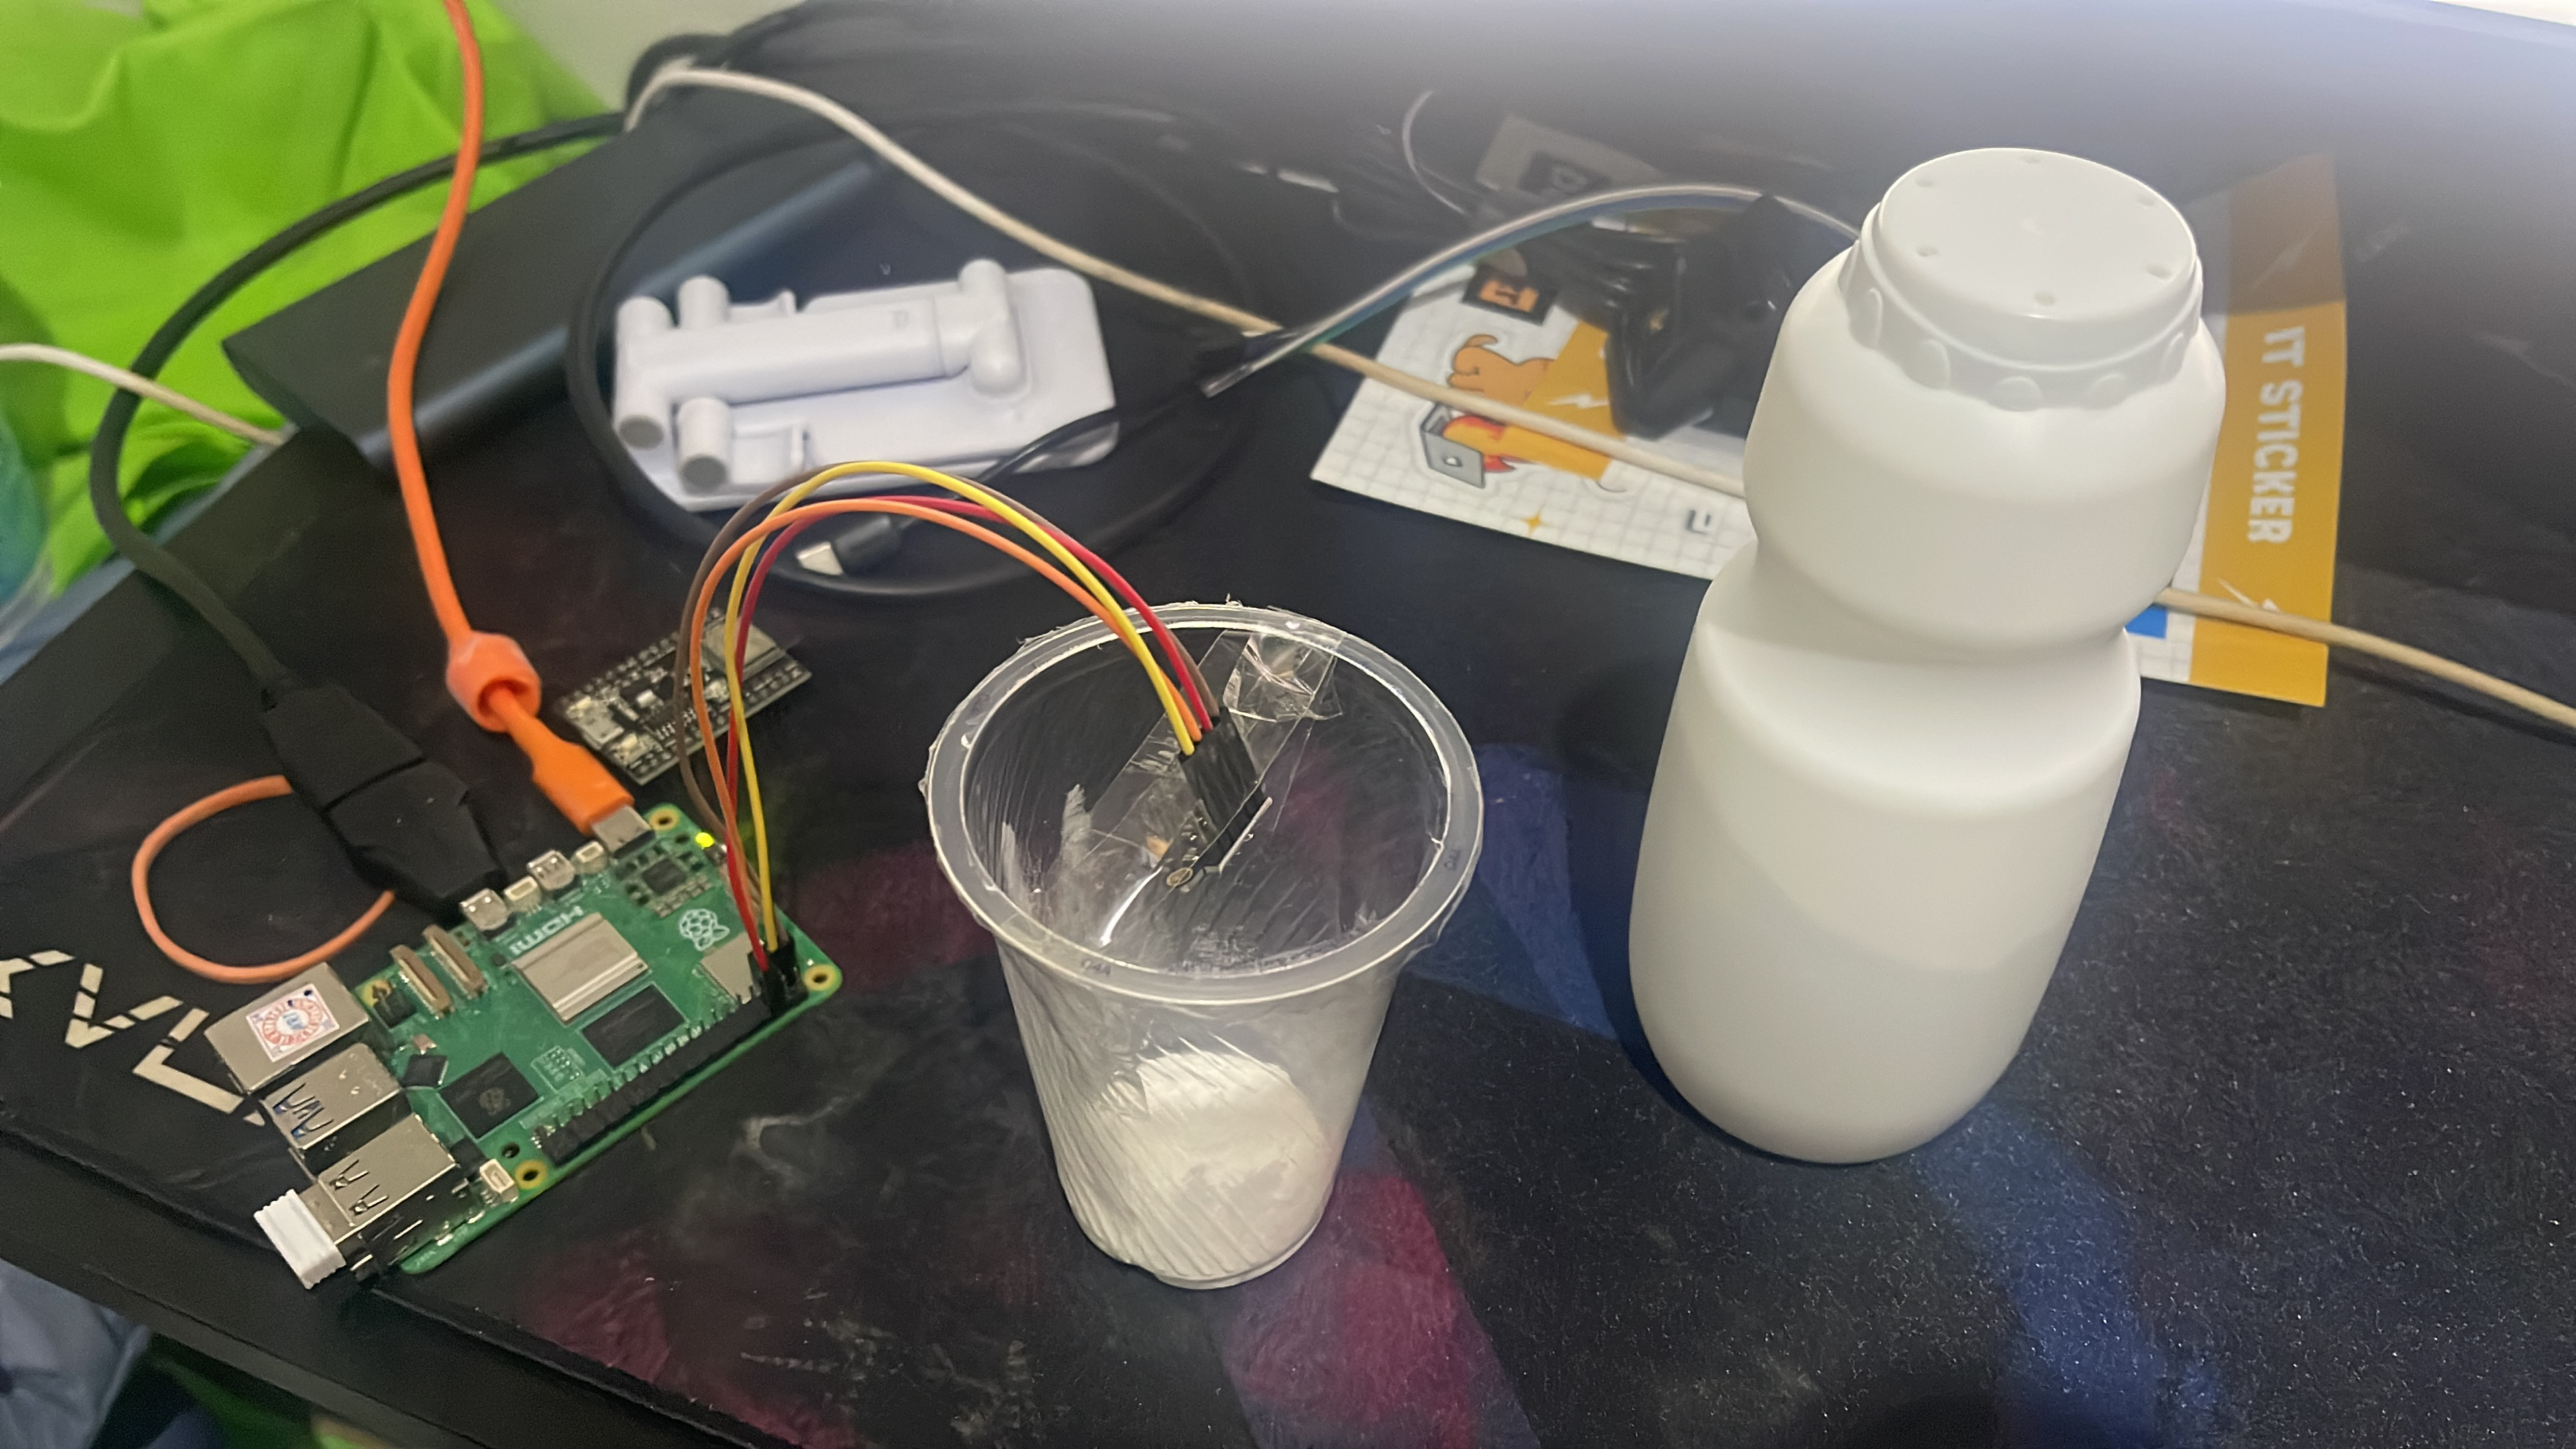
\includegraphics[width=0.6\textwidth]{gambar/sensor_0_persen.png}
  \caption{Pengujian Sensor saat Wadah Kosong (0\%)}
  \label{fig:sensor_0}
\end{figure}

\begin{figure}[H]
  \centering
  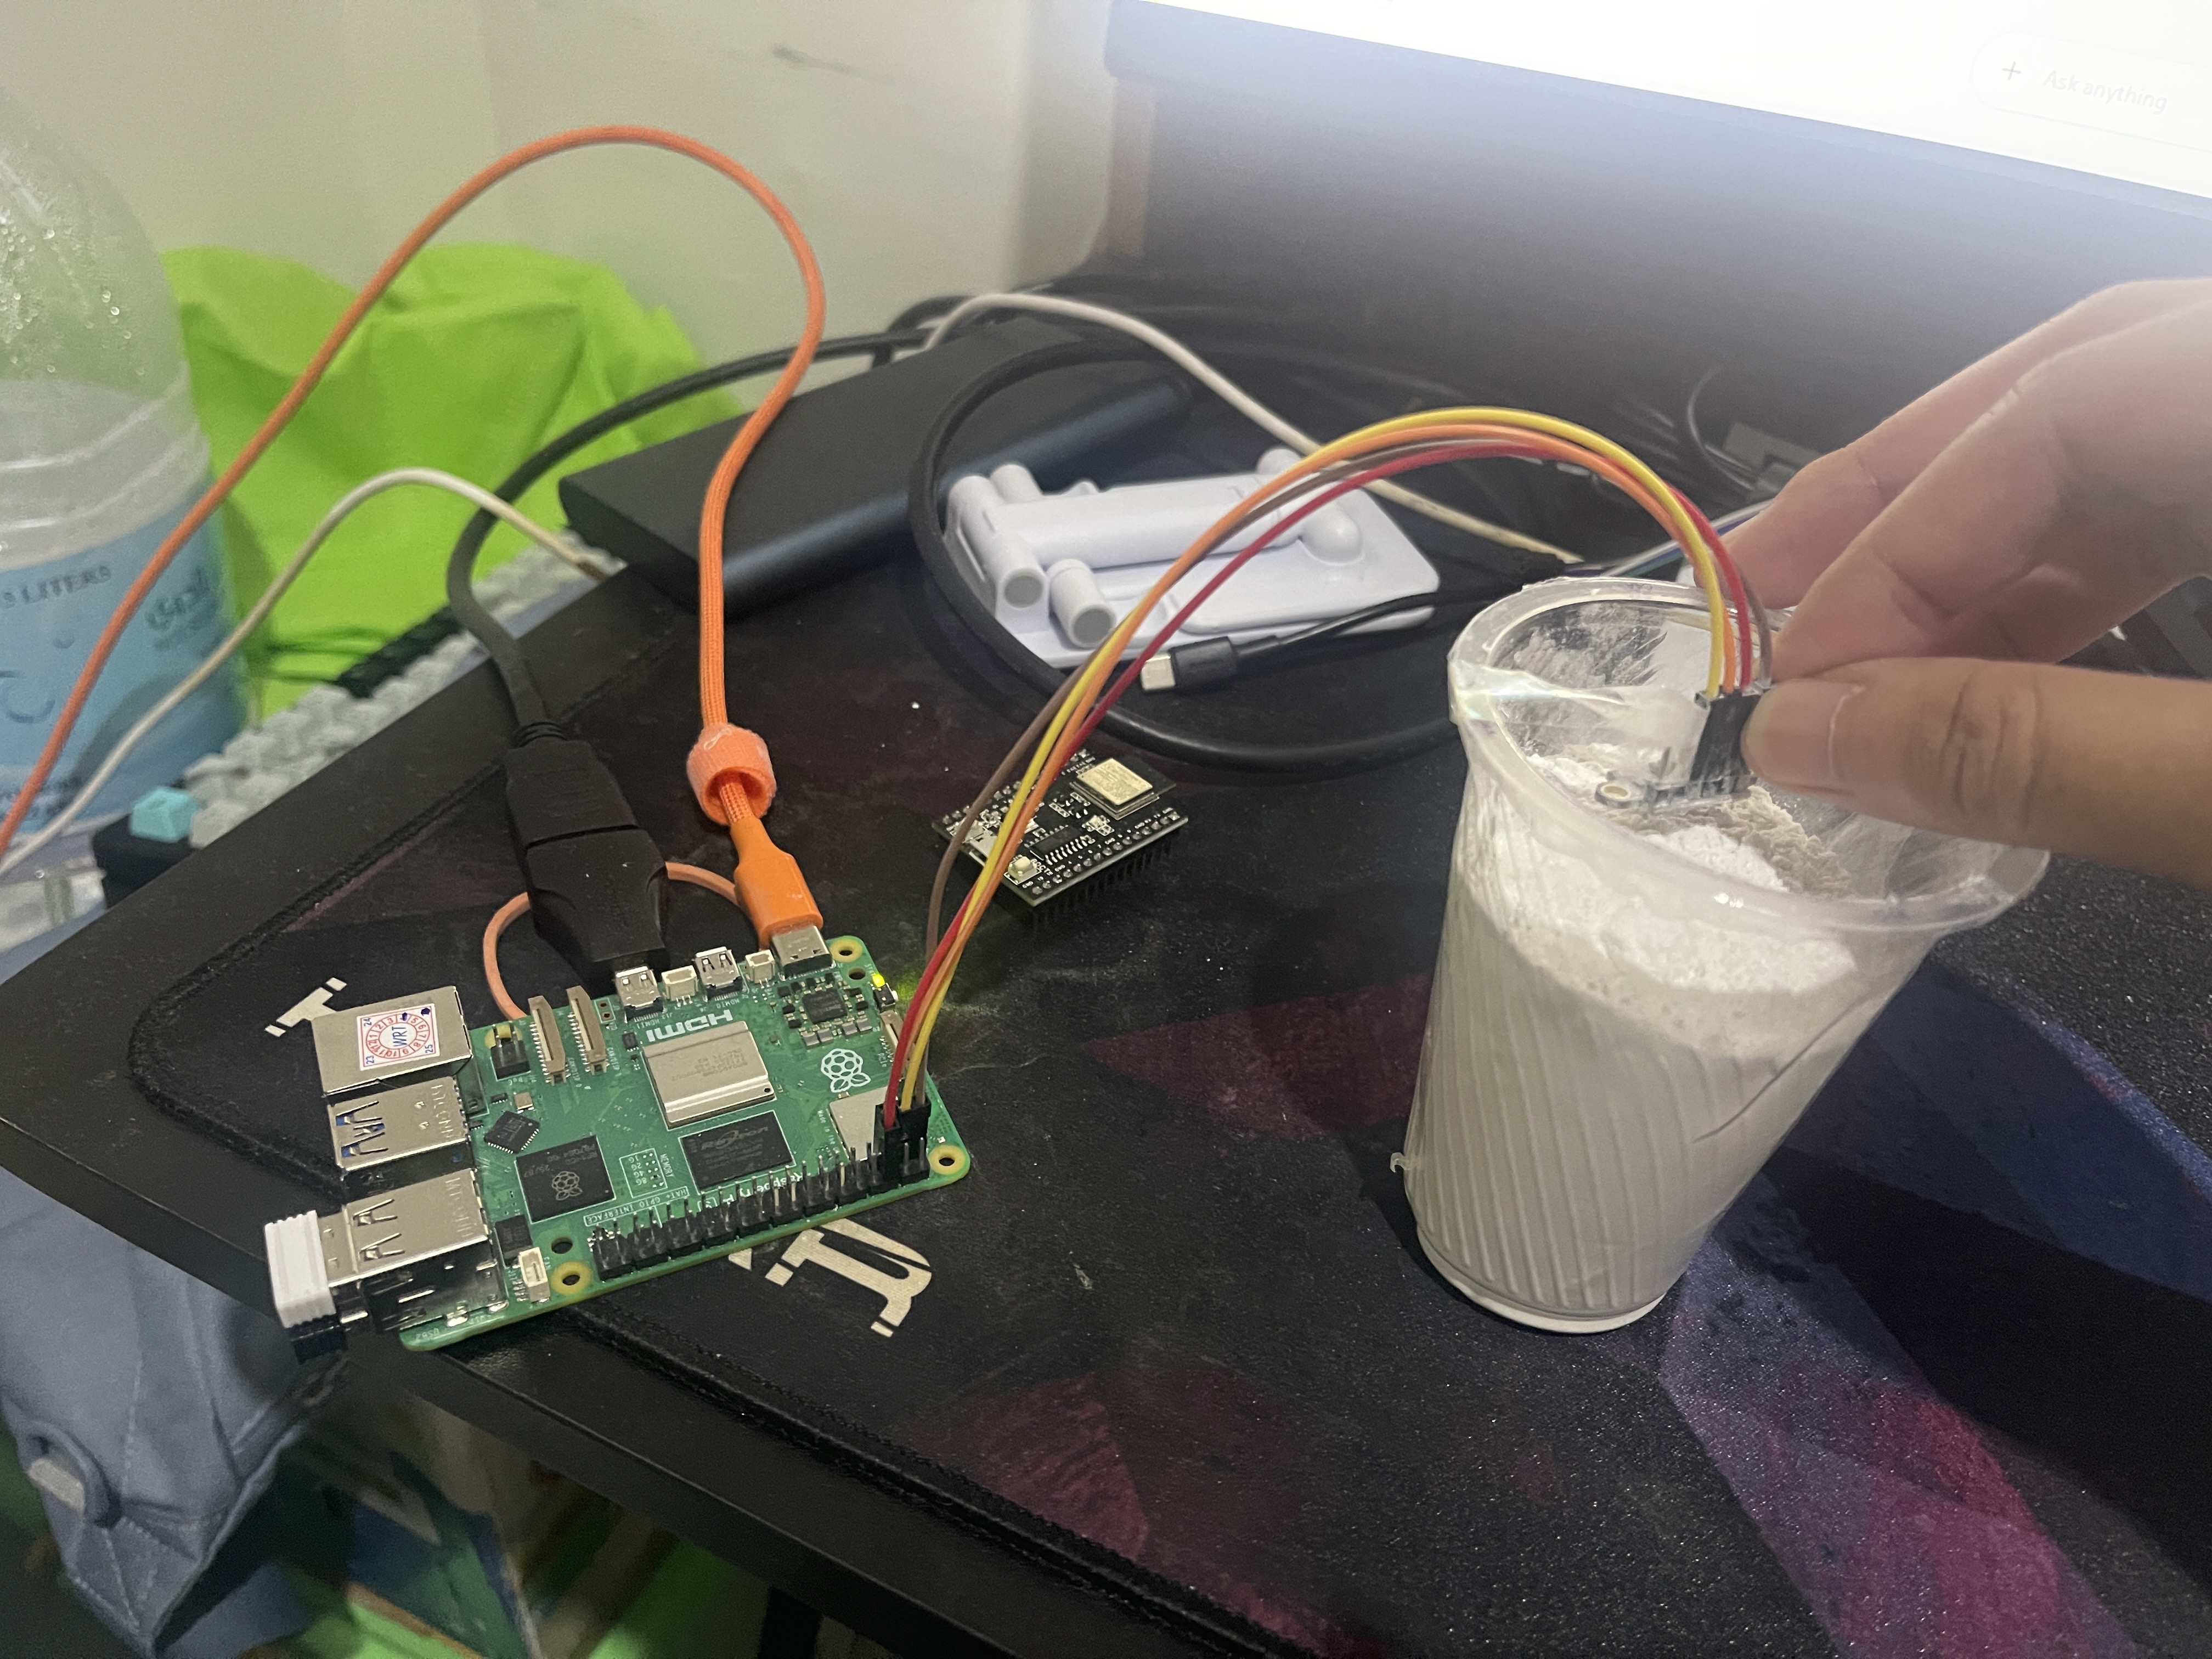
\includegraphics[width=0.6\textwidth]{gambar/sensor_100_persen.png}
  \caption{Pengujian Sensor saat Wadah Penuh (100\%)}
  \label{fig:sensor_100}
\end{figure}

Tabel \ref{tb:pengujian-vl53l0x} menunjukkan hasil pembacaan jarak mutlak sensor terhadap variasi volume serbuk di dalam wadah pengujian.

\begin{table}[H]
  \centering
  \caption{Hasil Pengujian Pembacaan Sensor VL53L0X}
  \label{tb:pengujian-vl53l0x}
  \begin{tabular}{|c|c|c|}
    \hline
    \rowcolor[HTML]{C0C0C0}
    \textbf{Kondisi Volume Aktual} & \textbf{Jarak Terbaca (mm)} & \textbf{Persentase Terukur (Mapping)} \\
    \hline
    0\% (Kosong) & 118 & 0.0\% \\
    25\% & 100 & 25.3\% \\
    50\% & 85 & 46.4\% \\
    75\% & 57 & 85.9\% \\
    100\% (Penuh) & 47 & 100.0\% \\
    \hline
  \end{tabular}
\end{table}

Berdasarkan hasil pengujian yang ditunjukkan pada Tabel \ref{tb:pengujian-vl53l0x}, jarak maksimum yang terukur saat wadah kosong (0\%) adalah 118 mm, sedangkan jarak minimum yang terukur saat wadah penuh (100\%) adalah 47 mm. Jarak 47 mm (4,7 cm) dipilih sebagai batas penuh (100\%) dan bukan menyentuh angka 0 mm untuk menghindari \emph{dead zone} (titik buta) sensor VL53L0X yang umumnya berada pada jarak kurang dari 30 mm, di mana pembacaan menjadi tidak valid atau memantul.

Oleh karena sensor membaca dalam bentuk jarak mutlak, maka nilai jarak tersebut harus dipetakan (\emph{mapping}) menjadi bentuk persentase kapasitas menggunakan interpolasi linear. Formula yang diterapkan dalam program untuk memproses data dari sensor adalah sebagai berikut:

\begin{equation}
  \text{Volume (\%)} = \left( \frac{\text{Jarak Kosong} - \text{Jarak Saat Ini}}{\text{Jarak Kosong} - \text{Jarak Penuh}} \right) \times 100
\end{equation}

Dengan memasukkan nilai batas maksimum dan minimum yang didapatkan dari pengujian, formulanya diturunkan menjadi:

\begin{equation}
  \text{Volume (\%)} = \left( \frac{118 - \text{Jarak Saat Ini}}{118 - 47} \right) \times 100
\end{equation}

Hasil \emph{mapping} menunjukkan nilai yang selaras pada persentase 25\% (terukur 25.3\%) dan mendekati pada 50\% (terukur 46.4\%). Namun, terdapat penyimpangan linieritas pada volume 75\% (terukur 85.9\%). Hal ini dianalisis terjadi akibat geometri wadah pengujian (gelas plastik) yang berbentuk kerucut terpancung (\emph{tapered}), sehingga penambahan volume secara fisik tidak berbanding lurus secara presisi dengan ketinggian serbuk. Meskipun demikian, algoritma pemetaan ini dinilai telah memvalidasi fungsionalitas pembacaan sensor dan akan menghasilkan tingkat linieritas yang lebih presisi apabila kelak diimplementasikan pada tabung penyimpanan \emph{pollen} berbentuk silinder sempurna yang telah disesuaikan dengan \emph{mount} pada \emph{drone}.



\section{Evaluasi Pengujian}
\label{sec:analisis-pengujian}

Dari pengujian yang \lipsum[1]

% Contoh pembuatan tabel
\begin{longtable}{|c|c|c|}
  \caption{Hasil Pengukuran Energi dan Kecepatan}
  \label{tb:energi-kecepatan}                                   \\
  \hline
  \rowcolor[HTML]{C0C0C0}
  \textbf{Energi} & \textbf{Jarak Tempuh} & \textbf{Kecepatan} \\
  \hline
  10 J            & 1000 M                & 200 M/s            \\
  20 J            & 2000 M                & 400 M/s            \\
  30 J            & 4000 M                & 800 M/s            \\
  40 J            & 8000 M                & 1600 M/s           \\
  \hline
\end{longtable}

\lipsum[2-4]
